\chapter{Análise Bibliográfica sobre Blockchains, por Bruno Sanguinetti Regadas de Barros\label{chap:bibliometria:Jaxiii}}

\section{Planejamento do estudo}

\textit{Blockchain}, ou em tradução livre , cadeia de blocos, A blockchain (também conhecido como “o protocolo da confiança”) é uma tecnologia de registro distribuído que visa a descentralização como medida de segurança. 
São bases de registros e dados distribuídos e compartilhados que têm a função de criar um índice global para todas as transações que ocorrem em um determinado mercado. Funciona como um livro-razão, só que de forma pública, compartilhada e universal, que cria consenso e confiança na comunicação direta entre duas partes, ou seja, sem o intermédio de terceiros.

Na atualidade, as \textit{Blockchains} são mais conhecidas pela sua aplicação em ferramentas monetárias e financeiras, como criptomoedas e NFTs. Porem as possibilidades de aplicações e análise de \textit{Blockchains} em áreas como logistica e IoT
também aparentam ser promissoras.


Partindo dos pontos acima, as questões que nortearam a pesquisa foram:
\begin{itemize}
    \item Quais são os tipo de \textit{Blockchains}?
    \item Quais as mantagens e desvantagens de cada tipo?
    \item Quais as aplicações de \textit{Blockchains} alem de moedas e NFTs? 
    \item Quais as implições éticas das aplicações de \textit{Blockchains}?
\end{itemize}

\subsection{Uso do Bibliometrix e Biblioshiny}
Serão usadas a ferramenta e o \textit{workflow} proposto pelos autores do pacote Bibliometrix, conforme indica a figura ~\ref{fig:bibliometrix:workflow}.

\subsection{Limitações} O exercício relatado foi feito em 4 horas e 20 minutos, utilizando a base de dados Web of Science (WoS)


\section{Coleta de dados\label{MASSA:coleta}}

A coleta de dados feita usando a base Web of Science (WoS) no dia 06 de fevereiro de 2022, acessado por meio do Portal de Periódicos da CAPES.

As buscas formam feitas nas coleções \textbf{Science  Citation  Index  Expanded (SCI -EXPANDED)} e \textbf{Social  Sciences  Citation  Index (SSCI)}, que contém registros relativos a vários campos do conhecimento, no qual o SCI-EXPANDED foca mais na área das ciências exatas e naturais, enquanto que o SSCI indexa artigos da área das ciências sociais. Observe que os artigos nessas duas coleções são indexados desde 1945. 

Foi usada a \textit{query} de busca ilustrada na listagem:

\lstinputlisting[numbers=left,basicstyle=\normalsize\ttfamily,caption={Query de busca sobre Blockchains.}]
{experiments/Jaxiii/PesquisaBibliometrica/Blockchains/query_01.txt}

\subsection{Explicação para os termos de busca usados}

A busca utilizou cláusulas que retornassem registros relacionados a \textit{Blockchain}. Evitando os registros que tratassem exclusivamente sobre notícias genericas, que não são pertinentes à análise. Os termos podem aparecer no título, no \textit{abstract} e/ou nas \textit{keywords}. 

Os termos \texttt{blockchain}, \texttt{smart-conctracts}, \texttt{iot}, \texttt{proof-of-work}, \texttt{proof-of-stake} buscam os resultados sobre \textit{Blockchains} e suas tecnologias derivadas. O termo \texttt{news} é utilizado para excluir os resultados que tratavam sobre notícias através de algoritmos de \textit{deep learning}.

Foram obtidos 1998 registros com a \textit{query} utilizada. Na exportação, foi utilizado o formato de arquivo de texto sem formatação, com os 29 campos disponíveis.

\section{Análise dos dados}

\subsection{Filtragem de registros}

O resultado do query resultou em quase todos os itens exportados sendo artigos, livros e \texttt{proceedings-papers}. O que gerou um \textit{dataset} satisfatório, sem necessidade de filtragem.

\subsection{Análise descritiva do \textit{dataset} }

A seguir, é feita uma análise bibliométrica descritiva do \textit{dataset} utilizando a função \texttt{biblioAnalysis} do Bibliometrix, que realiza diversos cálculos para levantar as taxas apresentadas.

As informações mais gerais sobre o \textit{dataset} são as seguintes:
\begin{description}
    \item [\textit{Timespan}] Os artigos filtrados foram publicados entre 2012 e 2022, o que indica que ainda há algum artigo não relacionado ao tema, que é relativamente recente.
    \item [\textit{Sources (Journals, Books, etc)}] São 611 fontes de informação que publicaram os artigos recuperados no \textit{dataset}.
    \item [\textit{Average years from publication}] A média do tempo de publicação dos artigos no \textit{dataset} é de 2,75 anos.
    \item [\textit{Average citations per documents}] Cada artigo no \textit{dataset} foi citado, em média 11,64 vezes.
    \item [\textit{Average citations per year per doc}] Após publicado, cada um dos artigos foi citado, em média, 2,699 vezes por ano.
    \item [\textit{References}] O \textit{dataset} contém 23591 referências citadas.
    \item [\textit{Keywords Plus (ID)}] 383 distintas palavras-chave do tipo Keywords Plus (ID) foram encontradas no \textit{dataset}.
    \item [\textit{Author's Keywords (DE)}] 2237 distintas palavras-chave indicadas pelos autores foram encontradas no \textit{dataset} .
    \item [\textit{Authors}] 3145 distintos nomes de autores foram encontrados no \textit{dataset} .
    \item [\textit{Author Appearances}] Os 3783 distintos (nomes de) autores foram encontrados 2.297 vezes, como autores de artigos.
    \item [\textit{Authors of single-authored documents}] Dentre os 93 distintos (nomes de) autores encontrados, 79 deles editaram artigos individualmente, isso é, sem co-autores.
    \item [\textit{Authors of multi-authored documents}] Dentre os 3052 distintos (nomes de) autores encontrados, 1.984 deles editaram artigos com um ou mais co-autores"
    \item [\textit{Single-authored documents}] Dentre os 97 documentos presentes no \textit{dataset}, 79 foram escritos por um único autor, e os restantes foram elaborados em co-autoria.
    \item [\textit{Documents per Author}] Dentre os 0.341 distintos (nomes de) autores, cada um publicou em média 0,26 artigos.
    \item [\textit{Authors per Document}] Cada um dos 2.93 documentos presentes no \textit{dataset} foi autorado com 3,84 autores em média.
    \item [\textit{Co-Authors per Documents}] As 3.53 aparições de (nomes de) autores (``Author Appearances''), sem distribuem, em média 4,28 vezes para os 537 documentos do \textit{dataset}.
    \item [\textit{Collaboration Index}] Os 3.13 (nomes de) autores que editaram artigos com um ou mais co-autores, colaboraram em media 4.28 vezes para editar os 537 artigos elaborados em co-autoria, gerando, assim, um índice de colaboração 4,33. 
\end{description}

\subsection{Evolução da Produção Científica}

\begin{figure}
    \centering
    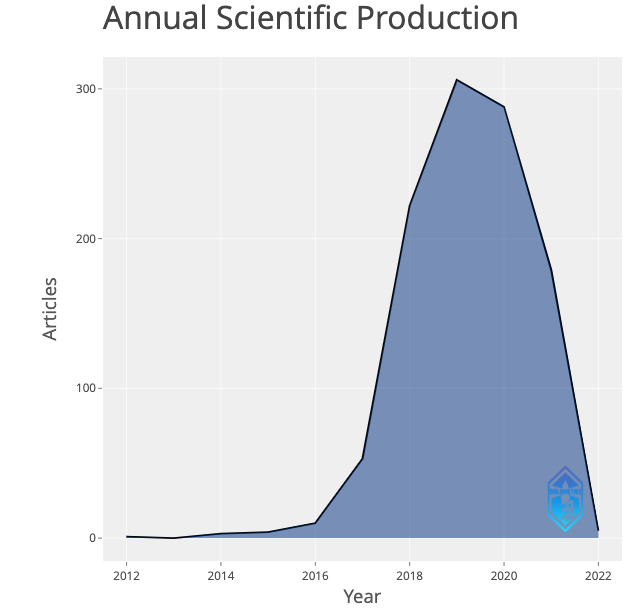
\includegraphics[width=1\textwidth]{experiments/Jaxiii/PesquisaBibliometrica/Blockchains/annual-plot.png}
    \caption{Evolução da produção científica no \textit{dataset}}
    \label{fig:evol:anual:blockchain@Jaxiii}
\end{figure}

A figura \ref{fig:evol:anual:blockchain@Jaxiii} representa a evolução em produção científica mundial a respeito do tema, de acordo com o \textit{dataset}. Apesar de nova, a produção tem um pico a partir do ano de 2018 até 2020, atingindo o pico em 2019. 

O \textit{Annual Growth Rate} do \textit{dataset} é consideravelmente alto entre os anos de 2015 e 2019, e de 19,58\% no acumulado dos anos.

\subsection{Interpretação do Crescimento} a taxa de crescimento do \textit{dataset} demonstra que o tema tem chamado muita atenção nos últimos anos, provavelmente devido à 
adoção de criptomoedas por parte da população e as possibilidades de aplicação de \textit{Blockchains}.

\subsection{Evolução das Citações}

\begin{figure}
    \centering
    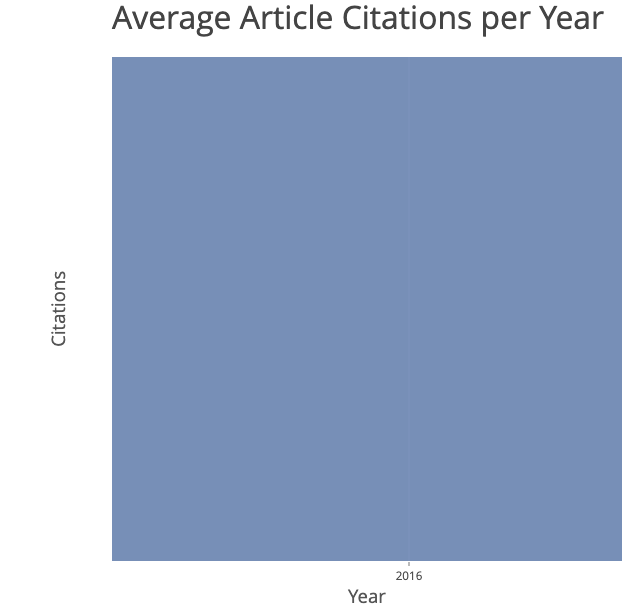
\includegraphics[angle=0,width=1\textwidth]{experiments/Jaxiii/PesquisaBibliometrica/Blockchains/citations-year-plot.png}
    \caption{Evolução das citações ao \textit{dataset}.}
    \label{fig:evol:anual:citacoes:blockchain@Jaxiii}
\end{figure}

A figura apresenta a evolução da média de citações aos artigos do \textit{dataset}. Não há muita estabilidade na média anual de citações, até mesmo nos anos mais recentes, que vem caindo.

\subsection{Interpretação das Citações}
As taxas inconstantes de citações por ano, e o crescimento abrupto do anos anteriores de publicações, pode demonstrar um tema ainda em sua infância.
\subsection{\textit{Three-Field Plots (Sankey diagram)}}

As \textit{Three-Field Plots (Sankey diagram)} (plotagens do tipo ``Três Campos'') correlacionam três conjuntos de atributos em busca das afinidades encontradas no \textit{dataset}. Assim, são demonstrados os principais fluxos entre diferentes conjuntos.

\begin{figure}
    \centering
    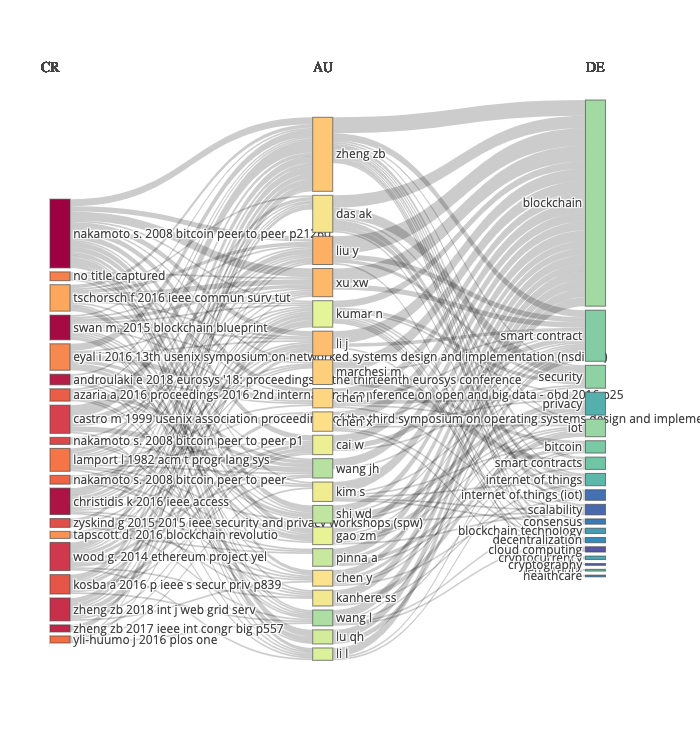
\includegraphics[width=1\textwidth]{experiments/Jaxiii/PesquisaBibliometrica/Blockchains/ThreeFieldPlot.png}
    \caption{Plotagem ``Três Campos'' (Sankey plot) do \textit{dataset}: 20 Autores, Citações e 20 Palavras-Chave mais proeminentes.}
    \label{fig:blockchain@Jaxiii:ThreeFieldPlot}
\end{figure}

A figura \ref{fig:blockchain@Jaxiii:ThreeFieldPlot} apresenta a plotagem do tipo ``Três Campos'' realizada no \textit{dataset}, vinculando, ao centro, os 20 Autores mais proeminentes (AU), à esquerda, as 20 Citações mais frequentes (CR - Cited Records), e à direita, as 14 Palavras-Chave mais frequentes empregadas pelos autores.

\subsection{Interpretação da figura \ref{fig:blockchain@Jaxiii:ThreeFieldPlot}}
A maioria dos autores mais relevantes apresentados na plotagem são, aparentemente, de origem oriental, mais especificamente chinesa e japonesa. Além disso, uma quantidade razoável dos artigos surgiram em universidades da China, EUA e Europa. O que sugere o avanço e o interesse do oriente a respeito do tema analisado.

É possível observar nas palavras-chave que há o surgimento do tema co-relacionado a temas de grande interesse público, como saúde e internet das coisas.
Os resultados sugerem que há interesse em estudar a aplicação de \textit{Blockchains} em temas de interesse comum.

\section{Refinamento da Coleta de Dados}

Após a análise do \textit{dataset}, foi possível notar que ainda existem poucas revisões e alta concentração de citações a um \textit{whitepaper}.

A analise de co-ocorrência, também demonstra que os temas estão bem co-relacionados e um refinamento não é necessario. Justificado também pela já
rasa fonte de dados.

\begin{figure}[htp]
    \centering
    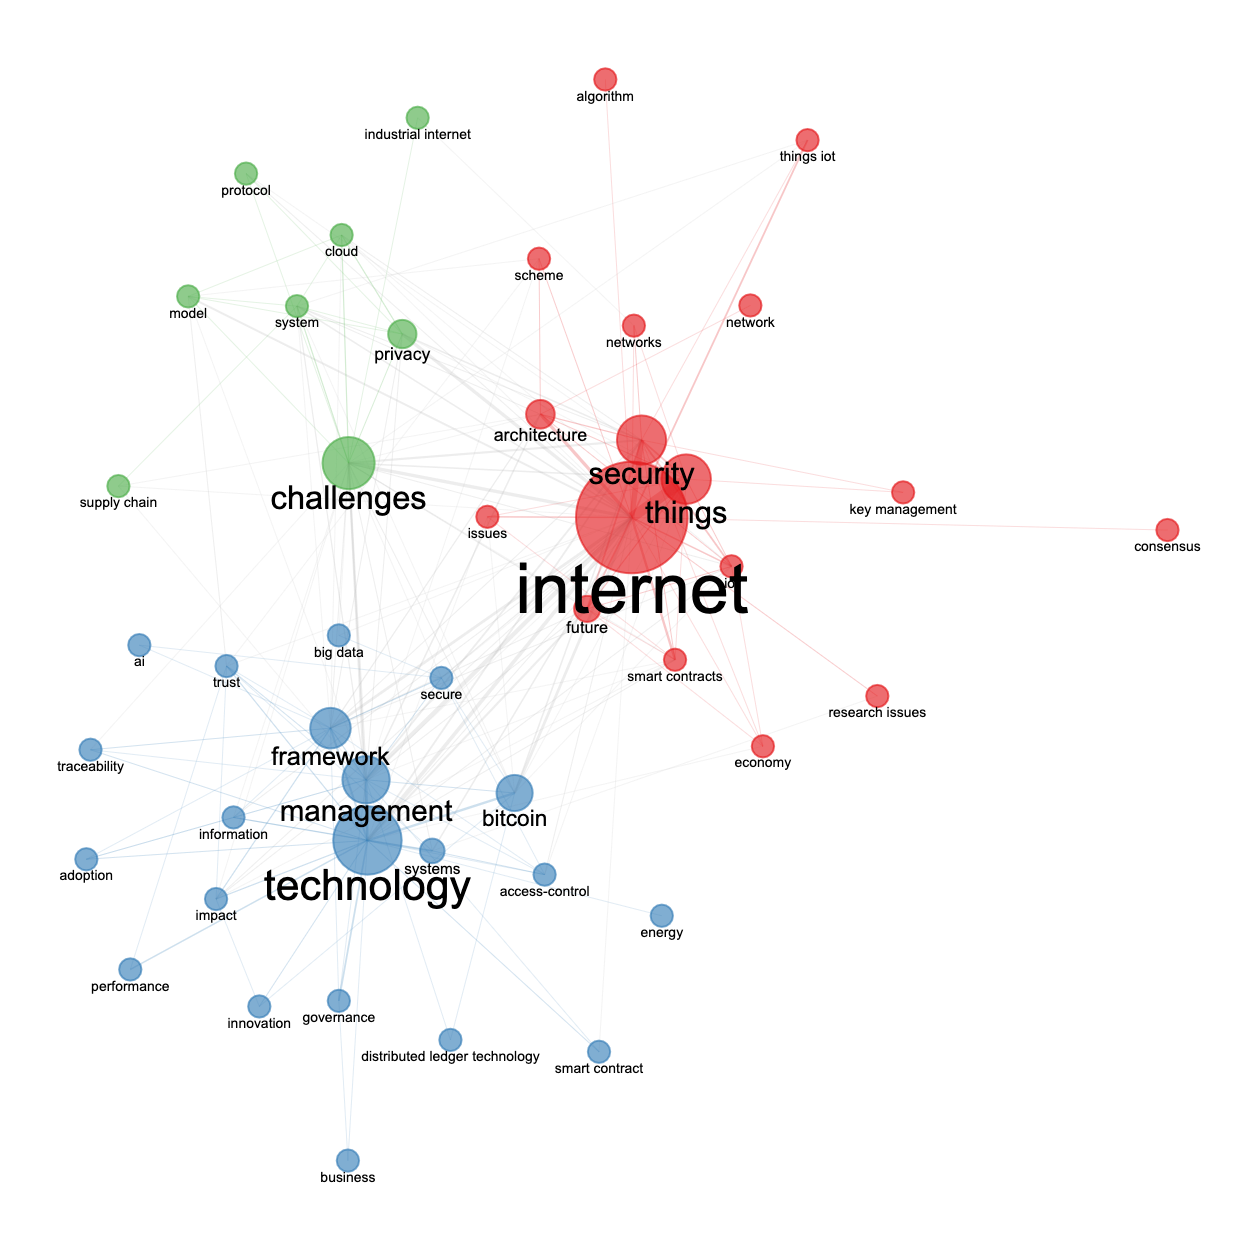
\includegraphics[width=0.6\textwidth]{experiments/Jaxiii/PesquisaBibliometrica/Blockchains/co-ocurrence.png}
    \caption{Rede de co-ocorrência de palavras aplicada ao \textit{dataset}.}
    \label{fig:blockchains@Jaxiii:redecoocorrencia}
\end{figure}

\subsection{Análise descritiva do \textit{dataset}}

\begin{table}[]
    \centering
\csvautotabular[separator=semicolon
%,filter not strcmp={\csvcolii}{}
]{experiments/Jaxiii/PesquisaBibliometrica/Blockchains/Most_Relevant_Sources.csv}
    \caption{Principais colaborações}
    \label{tab:blockchains:Main}
\end{table}

\subsection{Demais analises do \textit{dataset}}